\documentclass{beamer}

\usepackage{verbatim}
\usepackage{fancyvrb}
\usepackage{amsmath}
\usepackage{mathtools}
\usepackage{booktabs}
\usepackage{amssymb}
\usepackage{graphicx}
\usepackage{calc}
\usepackage{color}
\usepackage{multicol}
\usepackage{wrapfig}
\usepackage{natbib}
\usepackage[ruled,vlined]{algorithm2e}
\usepackage{animate}
\usepackage{mathtools}
\usepackage{listings}

\usepackage{cmbright}
\fontencoding{OT1}\fontfamily{cmbr}\selectfont %to load ot1cmbr.fd
\DeclareFontShape{OT1}{cmbr}{bx}{n}{% change bx definition
<->cmbrbx10%
}{}
\normalfont % back to normalfont

% two col: two columns
\newenvironment{twocol}[4]{
\begin{columns}[c]
\column{#1\textwidth}
#3
\column{#2\textwidth}
#4
\end{columns}
}

\makeatletter
\setbeamertemplate{theorem begin}
{%
\begin{\inserttheoremblockenv}
  {}{\usebeamerfont*{block title}\usebeamercolor[fg]{block title}%
  \inserttheoremname
  %\inserttheoremnumber
  \ifx \inserttheoremaddition \empty \else\ (\inserttheoremaddition)\fi
  \inserttheorempunctuation}
  \normalfont
  }
  \setbeamertemplate{theorem end}{\end{\inserttheoremblockenv}}
\makeatother

\newcommand{\E}{\mathrm{E}}
\newcommand{\Var}{\mathrm{Var}}
\newcommand{\Cov}{\mathrm{Cov}}
\newcommand{\sd}{\mathrm{sd}}
\newcommand{\s}{\mathrm{s}}
\newcommand{\Corr}{\mathrm{Corr}}
\newcommand{\rank}{\mathrm{rank}}
\newcommand{\trace}{\mathrm{trace}}
\newcommand{\nullspace}{\mathrm{null}}
\newcommand{\myspan}{\mathrm{span}}
\DeclareMathOperator*{\argmax}{arg\,max}
\DeclareMathOperator*{\argmin}{arg\,min}
\DeclareMathOperator*{\softmax}{softmax}

\definecolor{darkgreen}{rgb}{0,0.5,0}

\newtheorem{proposition}[theorem]{Proposition}
\newtheorem{exe}{Exercise}
\newtheorem{notation}{Notation}
\newtheorem{remark}{Remark}

\definecolor{darkgreen}{rgb}{0,0.5,0}
\title{Multiple Regression II}
\author{Zhenisbek Assylbekov}
\institute{Department of Mathematics}
\date{Regression Analysis}

\AtBeginSection[]
{
  \begin{frame}<beamer>
    \tableofcontents[currentsection]
  \end{frame}
}

\begin{document}

\begin{frame}
  \titlepage
\end{frame}

\section{Introduction}

\begin{frame}{Chapter 7 example: Body fat}
$n=20$ healthy females 25--34 years old.
\begin{itemize}
\item $x_1=$ triceps skinfold thickness (mm)
\item $x_2=$ thigh circumference (cm)
\item $x_3=$ midarm circumference (cm)
\item $Y=$ body fat (\%)
\end{itemize}

Obtaining $Y_i$, the percent of the body that is purly fat, requires
immersing a person in water. Want to develop model based on simple body measurements that avoids people getting wet.
\end{frame}

\begin{frame}{Scatterplot}
\centering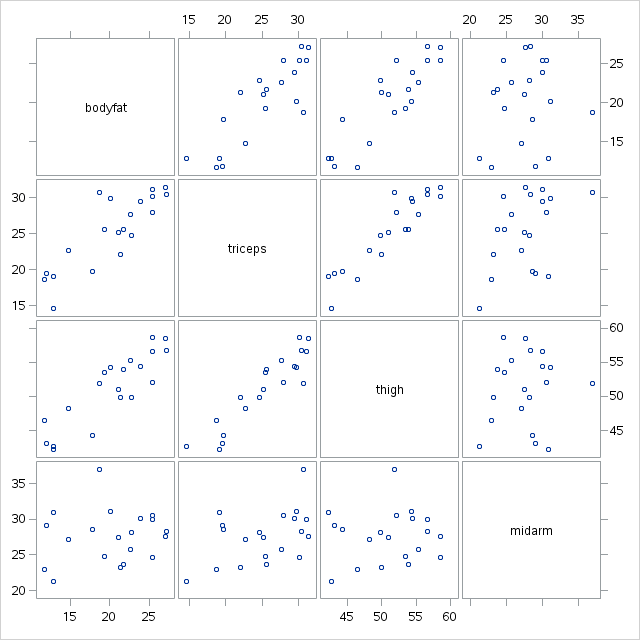
\includegraphics[scale=0.45]{plots/scatterplot}
\end{frame}

\begin{frame}{Correlation coefficients}
\begin{center}
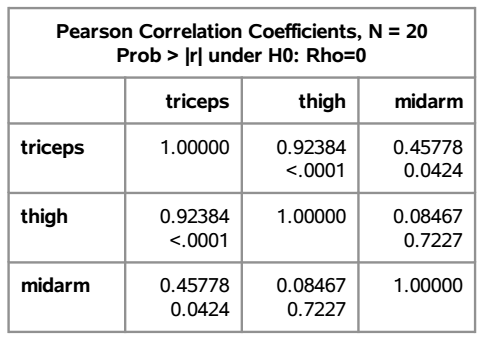
\includegraphics[scale=0.3]{plots/corr-matrix}
\end{center}

\pause There is high correlation among the predictors. \pause For example
$r = 0.92$ for triceps and thigh. These two variables are \textit{essentially
carrying the same information}. \pause Maybe only one or the other is really needed.
\vspace{10pt}

\pause In general, one predictor may be essentially perfectly predicted by
the remaining predictors (a high ``partial correlation''), and so would be unnecessary if the other predictors are in the model.
\end{frame}

\section{Extra sums of squares}

\begin{frame}{7.1 Extra sums of squares}
``Extra'' sums of squares are defined as the difference in SSE
between a model with some predictors and a larger model that
adds \textit{additional} predictors.
\vspace{10pt}

\pause \structure{Fact:} As predictors are added, the SSE can only decrease. \pause The
extra sums of squares is how much the SSE decreases:


\pause \begin{definition} Let $x_1, x_2, \ldots, x_k$ be predictors in a model.
\begin{multline}
{\rm SSR}(x_{j+1}, \ldots, x_k | x_1, x_2, \ldots, x_j) \\= {\rm SSE}(x_1, x_2, \ldots, x_j) - {\rm SSE}(x_1, x_2, \ldots, x_j, x_{j+1}, \ldots, x_k),
\end{multline}
\pause the difference in the sums of squared errors from the reduced to the full model.
\end{definition}

\pause This is how much of the total variation in SST is further explained by adding the new predictors.
\end{frame}

\begin{frame}{Example with $k=8$ predictors}
The predictors under consideration are
$$
x_1, x_2, x_3, x_4, x_5, x_6, x_7, x_8.
$$
\pause There are two models
\begin{align*}
\text{Reduced} &: x_1, x_3, x_5, x_6, x_8\\
\text{Full} &: x_1, x_2, x_3, x_4, x_5, x_6, x_7, x_8
\end{align*}
\vspace{-10pt}
\pause \begin{align*}
\text{Extra SS} &= {\rm SSR}(x_2, x_4, x_7|x_1, x_3, x_5, x_6, x_8)\\
& = {\rm SSE}(\text{reduced})-{\rm SSE}(\text{full})\\
& = {\rm SSE}(x_1, x_3, x_5, x_6, x_8) - {\rm SSE}(x_1, x_2, x_3, x_4, x_5, x_6, x_7, x_8)\\
& = {\rm SSR}(x_1, x_2, x_3, x_4, x_5, x_6, x_7, x_8) - {\rm SSR}(x_1, x_3, x_5, x_6, x_8)
\end{align*}
\pause This is how much \textit{additional} total variability (SST) is explained by adding $x_2, x_4, x_7$ to a model that already has $x_1, x_3, x_5, x_6, x_8$.
\end{frame}

\section{General linear test}

\begin{frame}{7.2 Associated tests}
We can formally test whether a certain set of predictors is useless,
\textit{in the presence} of other predictors in the model. \pause This is the \textit{general linear test}.\\~\\

\pause In the example above, we can test whether $x_2, x_4, x_7$ are needed if
$x_1, x_3, x_5, x_6, x_8$ are in the model.\\~\\
\pause If full (with
$x_1, x_2, x_3, x_4, x_5, x_6, x_7, x_8$) model has much lower SSE than reduced
model (without $x_2, x_4, x_7$) then at least one of $x_2, x_4, x_7$ is needed.
\end{frame}

\begin{frame}{F-test}
Say we want to test whether we can drop $q$ variables from a model
that has $p = k + 1$ (including the intercept), $q < p$.
\vspace{10pt}

\pause To test H$_0$: $\beta_{j_1} = \beta_{j_2} = \ldots = \beta_{j_q} = 0$ in the full model
\begin{align*}
F^\ast&=\frac{[{\rm SSE}(\text{reduced})-{\rm SSE}(\text{full})]/q}{{\rm SSE}(\text{full})/(n-p)}\\
&\sim F(q, n-p)
\end{align*}

\pause If H$_0$: $\beta_{j_1} = \beta_{j_2} = \ldots = \beta_{j_q} = 0$ is true; a p-value for the test is $\Pr(F^\ast > F_{q, n - p})$.
\vspace{10pt}

\pause Can be done in {\sc R}.
\end{frame}

\begin{frame}{F-test example with $k=8$ predictors}
To test H$_0$: $\beta_2=\beta_4=\beta_7=0$,
\begin{align*}
\onslide<2->{F^\ast &= \frac{[{\rm SSE}({\rm reduced})-{\rm SSE}({\rm full})]/(\text{\# params in test})}{{\rm MSE({\rm full})}}\\}
\onslide<3->{&=\frac{[{\rm SSE}(x_1, x_3, x_5, x_6, x_8)-{\rm SSE}(x_{1:8})]/3}{{\rm SSE}(x_{1:8})/(n-9)}\\}
\onslide<4->{&=\frac{{\rm SSR}(x_2, x_4, x_7|x_1, x_3, x_5, x_6, x_8)/3}{{\rm SSE}(x_{1:8})/(n-9)}\\}
\onslide<5->{&\sim F_{3,n-9}}
\end{align*}
\onslide<6->{if H$_0$: $\beta_2=\beta_4=\beta_7=0$ is true. ($x_{1:8}=x_1,x_2,\ldots,x_8$)}
\end{frame}

\begin{frame}[fragile]{Bodyfat example}{\url{https://github.com/zh3nis/MATH440/blob/main/chp07/bodyfat_extra_ss.R}}
\begin{small}
\begin{verbatim}
> anova(m_full, m_reduced)
Analysis of Variance Table

Model 1: bodyfat ~ triceps + thigh + midarm
Model 2: bodyfat ~ triceps + midarm
  Res.Df     RSS Df Sum of Sq      F Pr(>F)
1     16  98.405                           
2     17 105.934 -1   -7.5293 1.2242 0.2849
\end{verbatim}
\end{small}

\pause FTR H$_0:\beta_2=0$ in
$$
{\rm bodyfat}_i=\beta_0+\beta_1\times{\rm triceps}_i+\beta_2\times{\rm thigh}_i+\beta_3\times{\rm midarm}_i+\epsilon_i
$$
\end{frame}

\begin{frame}{Type I (sequential) sums of squares}
\begin{small}
Say you have $k=4$ predictors. Then the SSR for the full model can be written
\begin{align*}
{\rm SSR}&={\rm SSR}(x_1, x_2, x_3, x_4)\\
&={\rm SSR}(x_1)+{\rm SSR}(x_2|x_1)+{\rm SSR}(x_3|x_1, x_2)+{\rm SSR}(x_4|x_1, x_2, x_3).
\end{align*}
These are called \textbf{sequential sums of squares}, or Type I sums of squares. They explain how much variability is absorbed by adding predictors sequentially to a model. There are four corresponding hypothesis tests with these sequential sums of squares:
\end{small}
\vspace{-10pt}

\begin{table}[h]
\begin{center}
\begin{small}
\begin{tabular}{l l l}
Model & Hypothesis & F-statistic\\
\hline
$Y_i=\beta_0+\beta_1 x_{i1}+\epsilon_i$ & H$_0:\beta_1=0$ & $\frac{{\rm MSR}(x_1)}{{\rm MSE}(x_1)}$\\
$Y_i=\beta_0+\beta_1 x_{i1}+\beta_2 x_{i2}+\epsilon_i$ & H$_0:\beta_2=0$ & $\frac{{\rm MSR}(x_2|x_1)}{{\rm MSE}(x_1,x_2)}$\\
$Y_i=\beta_0+\beta_1 x_{i1}+\beta_2 x_{i2}+\beta_3 x_{i3}+\epsilon_i$ & H$_0:\beta_3=0$ & $\frac{{\rm MSR}(x_3|x_1,x_2)}{{\rm MSE}(x_1,x_2,x_3)}$\\
$Y_i=\beta_0+\beta_1 x_{i1}+\beta_2 x_{i2} + \beta_3 x_{i3}+\beta_4 x_{i4}+\epsilon_i$ & H$_0:\beta_4=0$ & $\frac{{\rm MSR}(x_4|x_1,x_2,x_3)}{{\rm MSE}(x_1,x_2,x_3,x_4)}$
\end{tabular}
\end{small}
\end{center}
\end{table}
\end{frame}

\begin{frame}[fragile]
\frametitle{Sequential SS in {\sc R} --- Bodyfat example}
\begin{small}
\begin{verbatim}
> anova(m_full)
Analysis of Variance Table

Response: bodyfat
          Df Sum Sq Mean Sq F value    Pr(>F)    
triceps    1 352.27  352.27 57.2768 1.131e-06 ***
thigh      1  33.17   33.17  5.3931   0.03373 *  
midarm     1  11.55   11.55  1.8773   0.18956    
\end{verbatim}

\begin{itemize}
\item<2-> Reject H$_0:\beta_1=0$ in ${\rm fat}_i=\beta_0+\beta_1\times{\rm triceps}_i+\epsilon_i$
\item<3-> Reject H$_0: \beta_2=0$ in ${\rm fat}_i=\beta_0+\beta_1\times{\rm triceps}_i+\beta_2\times{\rm thigh}_i+\epsilon_i$
\item<4-> FTR H$_0:\beta_3=0$ in ${\rm fat}_i=\beta_0+\beta_1\times{\rm triceps}_i+\beta_2\times{\rm thigh}_i+\beta_3\times{\rm midarm}_i+\epsilon_i$
\item<5-> Order entered (triceps, thigh, midarm) matters!
\end{itemize}
\end{small}
\end{frame}

\begin{frame}{ANOVA table \& decomposing the SSR(F)}
\begin{center}
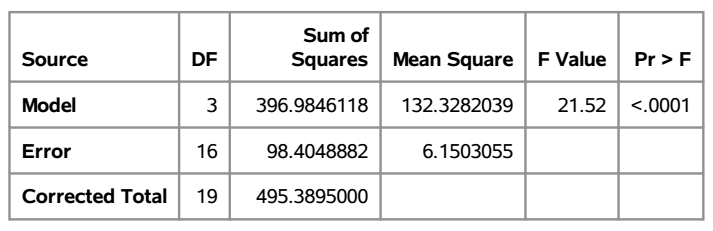
\includegraphics[scale=0.25]{plots/anova}
\end{center}
The sequential extra sums of squares are given on the previous slide:\\~\\
SSR$(x_1) = 352.3$; SSR$(x_2|x_1) = 33.2$, and SSR$(x_3 |x_1 , x_2) = 11.5$.\\~\\

\pause Almost all of the SSR$(x_1 , x_2 , x_3 ) = 397.0$ is explained by $x_1$
(triceps) alone.\\~\\
\pause Also note, as required,
\begin{multline*}
{\rm SSR}(x_1, x_2, x_3) = 397.0 = 352.3+33.2+11.5\\ = {\rm SSR}(x_1)+{\rm SSR}(x_2|x_1)+{\rm SSR}(x_3| x_1, x_2).
\end{multline*}
\end{frame}


\section{Coefficients of partial determination}

\begin{frame}{7.4 Coefficients of partial determination}
We can {\it standardize} extra sums of squares to be between 0 and 1.\\~\\

\pause The \textbf{coefficient of partial determination} is the fraction by which the SSE is reduced when adding new predictor(s) to an existing model. \pause Examples:
\begin{itemize}
\item\pause $R^2_{Y2\mid1}={\rm SSR}(x_2\mid x_1)/{\rm SSE}(x_1)$
\item\pause $R^2_{Y3\mid12}={\rm SSR}(x_3\mid x_1,x_2)/{\rm SSE}(x_1,x_2)$
\item\pause $R^2_{Y23\mid1}={\rm SSR}(x_2,x_3\mid x_1)/{\rm SSE}(x_1)$\\~\\
\end{itemize}


\pause For example, if $R^2_{Y3|12}=0.5$ then {\it 50\% of the remaining variability} is explained by adding $x_3$ to a model that already had $x_1$ and $x_2$.
\end{frame}

\begin{frame}[fragile]{Partial $R^2$ in {\sc R} --- Bodyfat example}
\begin{verbatim}
> library(rsq)
> m_midarm_only = update(m_full, . ~ . - triceps - thigh)
> m_midarm_triceps = update(m_full, . ~ . - thigh)
> rsq.partial(m_midarm_triceps, m_midarm_only)
$adjustment
[1] FALSE

$variables.full
[1] "triceps" "midarm" 

$variables.reduced
[1] "midarm"

$partial.rsq
[1] 0.7817311
\end{verbatim}
\end{frame}


\section{Multicollinearity}

\begin{frame}[fragile]{7.6 Multicollinearity}
\begin{footnotesize}
\begin{verbatim}
> summary(m_full)

Call:
lm(formula = bodyfat ~ triceps + thigh + midarm, data = bodyfat_data)
...

Coefficients:
            Estimate Std. Error t value Pr(>|t|)
(Intercept)  117.085     99.782   1.173    0.258
triceps        4.334      3.016   1.437    0.170
thigh         -2.857      2.582  -1.106    0.285
midarm        -2.186      1.595  -1.370    0.190

Multiple R-squared:  0.8014,	Adjusted R-squared:  0.7641 
F-statistic: 21.52 on 3 and 16 DF,  p-value: 7.343e-06
\end{verbatim}
\end{footnotesize}

\pause We reject
H$_0: \beta_1 = \beta_2 = \beta_3 = 0$, BUT we fail to reject $\text{H}_0:\,\beta_j=0$ individually!
\end{frame}

\begin{frame}{7.6 Multicollinearity}
The set $x_1$, $x_2$, $x_3$ are useful for explaining body fat, but none of
the three are useful in the presence of the other two.
\vspace{10pt}

\textbf{Why?} \pause The predictors are measuring similar phenomena; their
sample values are highly correlated. \pause For example, $r = 0.924$ between triceps thickness $x_1$ and thigh circumference $x_2$.
\vspace{10pt}

\pause This is known as \alert{multicollinearity} among the predictors.
\end{frame}

\begin{frame}{Effects of multicollinearity}
\begin{itemize}
\item<2-> Model may still provide a good fit and precise
prediction/estimation of the response.
\item<3-> Several estimated regression coefficients $b_1$, $b_2$, \ldots , $b_k$ will
have large standard errors (pp.~281--283), leading to conclusions that
individual predictors are \textit{not significant} although overall F-test
may be \textit{highly} significant.
\item<4-> Concept of ``holding all other predictors constant'' doesn’t
make sense in practice.
\item<5-> Signs of regression coefficients may be ``opposite'' of intuition
(or what we might think \textit{marginally} they might be based on a scatterplot).
\end{itemize}
\end{frame}

\begin{frame}[fragile]
\frametitle{Bodyfat example}
\begin{small}
\begin{verbatim}
lm(formula = bodyfat ~ triceps + thigh + midarm, 
   data = bodyfat_data)

Coefficients:
            Estimate Std. Error t value Pr(>|t|)
(Intercept)  117.085     99.782   1.173    0.258
triceps        4.334      3.016   1.437    0.170
thigh         -2.857      2.582  -1.106    0.285
midarm        -2.186      1.595  -1.370    0.190
\end{verbatim}
\end{small}

\pause Two of the three regression effects are {\it negative}. \pause Holding midarm
and triceps constant, increasing the thigh circumference 1 mm
{\it decreases} bodyfat. \pause Does this make sense?
\end{frame}

\begin{frame}{Detecting multicollinearity}
Predictor $x_j$ has a \textit{variance inflation factor} of
$$
VIF_j=\frac{1}{1-R^2_j},
$$
where $R^2_j$ is the $R^2$ from regressing $x_j$ on the remaining predictors $x_1,x_2,\ldots,x_{j-1},x_{j+1},\ldots,x_k$.\\~\\

\pause High $R^2_j$ (near 1) $\Rightarrow$ $x_j$ is linearly associated with other predictors $\Rightarrow$ high $VIF_j$.\\~\\

\begin{itemize}
\item\pause $VIF_j\approx1\Rightarrow x_j$ is not involved in any multicollinearity.
\item\pause $VIF_j>10\Rightarrow x_j$ is involved in severe multicollinearity.
\end{itemize}
\end{frame}

\begin{frame}[fragile]{VIF$_j$'s in {\sc R}}
\begin{verbatim}
> library(car)
> vif(m_full)
 triceps    thigh   midarm 
708.8429 564.3434 104.6060 
\end{verbatim}

What do you conclude?
\end{frame}

\begin{frame}{Remedies of multicollinearity}
\begin{itemize}
\item Drop one or more predictors from the model. We'll discuss this in Chapter 9.
\item<2-> More advanced: \textit{principle components regression} uses new predictors that are linear combinations of the
original predictors as predictors in a new model. The new predictors
are selected to be uncorrelated. Disadvantage: the new predictors
might be hard to interpret.
\item<3-> More advanced: \textit{ridge regression} (Section 11.2).
\end{itemize}


\end{frame}

\end{document}